\section{Debugging della rete}
Una volta che avrete progettato la vostra rete ed avrete impostato i vari dispositivi, avrete la necessità di controllare se sono presenti vari errori nella rete, a questo scopo esiste il debugging della rete, ovvero il controllo degli eventuali errori.

In questa sezione del documento saranno trattati i seguenti argomenti:

\begin{itemize}
    \item Gli indirizzi IP assegnati e lo stato delle porte (IPV4 e IPV6)
    \item La sintesi delle tabelle di routing
    \item La verifica tramite ping
    \item La verifica tramite simulation
\end{itemize}

\subsection{Indirizzi IP assegnati e stato delle porte (IPv4 e IPv6)}
Nel caso vogliate visualizzare gli indirizzi ip assegnati e lo stato delle porte, dovrete scrivere nella console del router di vostro interesse il comando show run (in forma estesa significherebbe show running -config), in questo modo potrete visualizzare le informazioni citate prima.

\begin{center}
    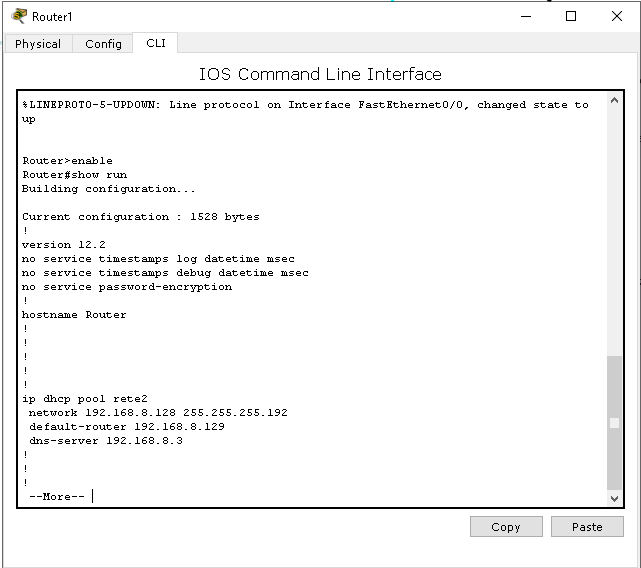
\includegraphics[width=\linewidth]{images/04.debugging-rete/01.png}
\end{center}

Se si presenta la scritta shutdown nell’ output, significa che la porta non è funzionante, vi ricordo che ogni volta che assegnate un indirizzo ip è necessario scrivere il comando no shutdown, come ultimo comando, per rendere la porta funzionante.

Lo stato delle porte all'inizio (dopo aver eseguito il comando no shutdown) richiede tempo prima che siano pronte per solvere il loro compito, se si vuole velocizzare la procedura basta cliccare sul bottone Capture/Forward (in alcuni casi sopra ci può essere scritto Fast Forward) presente nella parte in basso nella riga gialla.

\begin{center}
    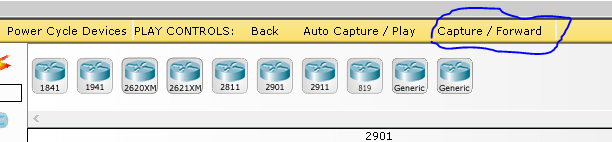
\includegraphics[width=\linewidth]{images/04.debugging-rete/02.png}
\end{center}

Le informazioni riguardanti la configurazione (quelle date in output con lo show running config) non vengono memorizzate in modo automatico, per fare in modo che vengano salvate potete usare il comando save running config, il quale vi consentirà il loro salvataggio.

Un altro comando che vi può risultare utile è il comando show ip interface brief, il quale darà in output

I vari indirizzi assegnati alle varie interfacce disponibili, inoltre potrete avere in output anche lo stato delle interfacce. 

\begin{center}
    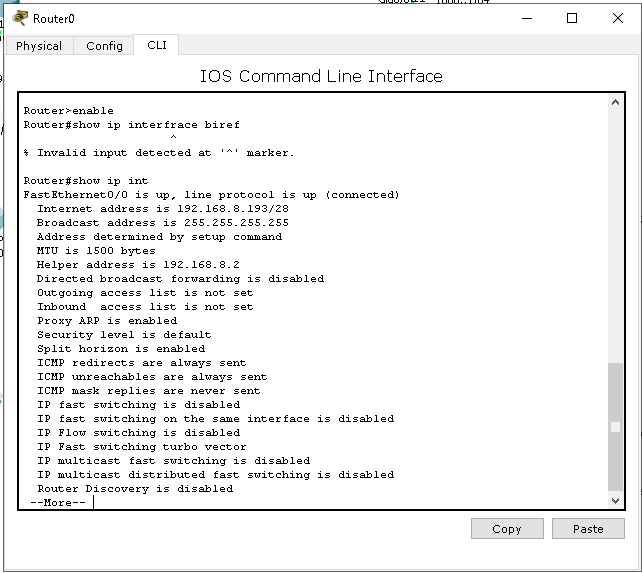
\includegraphics[width=\linewidth]{images/04.debugging-rete/03.png}
\end{center}

\subsection{Sintesi tabelle di routing}

Nel caso si voglia visualizzare la sintesi della tabella di routing del router bisogna fare doppio click sul router di nostro interesse, accedere alla console, digitare il comando enable(ena) e scrivere la seguente riga di codice: \emph{netstat -r}.

Una volta che si è svolta tale procedura si potrà visualizzare la tabella nella console in questo modo:

\begin{verbatim}
Routing tables
Destination      Gateway         Flags     Refs   Use       Interface

Route Tree for Protocol Family 2:
default          194.20.20.6     UG        196    18646259  tu0
127.0.0.1        127.0.0.1       UH        2      27417     lo0
194.20.20        194.20.20.20    U         190    44212849  tu0
192.36.73        194.20.20.6     UGDM      0      33189     tu0
193.45.68        194.20.20.32    UGD       0      91719     tu0
193.45.71        194.20.20.33    UGD       0      6484      tu0
194.20.20.211    194.20.20.7     UGHD      0      7508      tu0
\end{verbatim}

I vari flags che ci si presentano hanno ognuno un significato in particolare:

\begin{itemize}
    \item \textbf{U} significa che la route è attiva (UP)
    \item \textbf{G} significa che la route è tramite un gateway
    \item \textbf{H} significa che la route è verso un host
    \item \textbf{D} significa che la route è stata creata da un ICMP redirect
    \item \textbf{M} significa che la route è stata modificata da un ICMP redirect
\end{itemize}

Come si può vedere dalla tabella, le varie flags si mostrano unite tra loro, ovvero che ogni dato presente nella tabella ci sono più opzioni riguardanti la flag.

Il campo refs indica il numero di connessioni TCP in uso, mentre il campo use indica il numero di pacchetti trasferiti.

Se si vuole esaminare le informazioni della tabella di routing bisogna inserire, nella console ,il comando show ip route, il quale darà un output simile a questo:

\begin{fcmds}{Priviledged mode}
    \$ show ip route
\end{fcmds}

\begin{verbatim}
Codes: C - connected, S - static, I - IGRP, R - RIP, M - mobile, B – BGP
D - EIGRP, EX - EIGRP external, O - OSPF, IA - OSPF inter area 
E1 - OSPF external type 1, E2 - OSPF external type 2, E – EGP
i - IS-IS, L1 - IS-IS level-1, L2 - IS-IS level-2, * - candidate default
Gateway of last resort is 0.0.0.0 to network 0.0.0.0
D    194.21.195.0 [90/40537600] via 194.20.20.36, 00:01:06, Ethernet0
D    194.20.194.0 [90/281600] via 194.20.20.35, 17:46:12, Ethernet0
D    194.20.195.0 [90/281600] via 194.20.20.35, 17:46:12, Ethernet0
D    194.20.192.0 [90/281600] via 194.20.20.35, 17:46:14, Ethernet0
D    194.20.193.0 [90/281600] via 194.20.20.35, 17:46:12, Ethernet0
S    194.20.146.0 is directly connected, Serial0
S    194.20.147.0 is directly connected, Serial0
S    194.20.144.0 is directly connected, Serial0
     194.20.145.0 is variably subnetted, 2 subnets, 2 masks
S   194.20.145.0 255.255.255.0 is directly connected, Serial0
C   194.20.145.252 255.255.255.252 is directly connected, Serial0
     194.20.158.0 is variably subnetted, 2 subnets, 2 masks
S   194.20.158.0 255.255.255.0 is directly connected, Serial2
C   194.20.158.240 255.255.255.240 is directly connected, Serial2
S    194.20.159.0 is directly connected, Serial2
S    194.20.156.0 is directly connected, Serial2
\end{verbatim}

Le informazioni più dettagliate riguardanti una singola route si possono avere eseguendo il comando show ip route più l'indirizzo sulla console, usando questo comando si potrà ottenere un output simile a questo:

\begin{fcmds}{Priviledged mode}
    \$ show ip route 194.21.195.0
\end{fcmds}

\begin{verbatim}
Routing entry for 194.21.195.0 255.255.255.0
Known via "eigrp 1", distance 90, metric 40537600, type internal
Redistributing via eigrp 1
Last update from 194.20.20.36 on Ethernet0, 00:01:37 ago
Routing Descriptor Blocks:
194.20.20.36, from 194.20.20.36, 00:01:37 ago, via Ethernet0
Route metric is 40537600, traffic share count is 1
Total delay is 21000 microseconds, minimum bandwidth is 64 Kbit
Reliability 255/255, minimum MTU 1500 bytes
Loading 3/255, Hops 1
\end{verbatim}

\subsection{Verifica tramite Ping}
Un secondo metodo per controllare se la vostra rete comunichi o meno, è la verifica tramite ping.

Il ping è un comando che consente di inviare i pacchetti ad un altro dispositivo della rete grazie al suo indirizzo ip, in questo modo se il destinatario riceve i pacchetti la parte di rete che serve per la comunicazione tra i dispositivi in questione funziona, altrimenti c'è qualche problema a cui bisogna rimediare.

Prendiamo ora il caso ipotetico che un pc debba comunicare con un altro pc (dobbiamo far comunicare il PC1 con il PC2).

Una volta che conosciamo l'indirizzo ip del PC2 bisogna preoccuparsi di inserirlo nel command prompt presente nel PC1 con l’apposito comando, in altre parole, una volta che ci troviamo nella schermata nera del command prompt dobbiamo scrivere il comando ping più l’indirizzo ip, ovvero: ping 192.168.1.1 (l'indirizzo ip è solo un esempio, voi dovete inserire l'ip del PC2).

Una volta eseguito il comando ci si presenteranno delle righe simili a questa questa: Reply from 192.168.1.1: byte=32 time=125ms TTL=128, queste righe descrivono l'invio dei pacchetti, nel caso la struttura delle righe sia identica a questa, ovviamente con valori numerici differenti, il comando ping è andato a buon fine , in caso contrario ci sono dei problemi da risolvere.

\subsection{Verifica tramite simulation}
Un'altra tipologia di verifica è quella della simulazione o simulation, la quale consente di simulare il funzionamento della rete.

In basso a destra potrete notare due icone una appoggiata sull' altra, dovete cliccare su quella che si presenta sopra rispetto all'altra, una volta che avrete cliccato sarete passati dalla modalità real time alla modalità simultation.

\begin{center}
    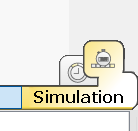
\includegraphics[width=\linewidth]{images/04.debugging-rete/04.png}
\end{center}

E’ necessario anche selezionare soltanto i protocolli legati alle funzioni che dovete eseguire, questa operazione si attua entrando nella event list, poi bisogna selezionare show all none in modo che si formatti tutta la event list ed infine cliccare solo sui protocolli che vi servono, in questo caso vi serve solamente l'ICMP.

\begin{center}
    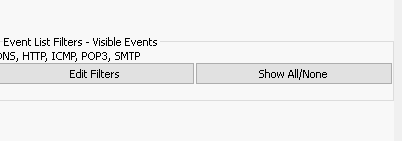
\includegraphics[width=\linewidth]{images/04.debugging-rete/05.png}
\end{center}

Nella parte dello schermo relativa alla tool box di cisco bisogna cliccare nell’ opzione add simple PDU, ovvero l'icona che si presenta come una busta chiusa con il simbolo del più, poi dovete cliccare sul dispositivo di rete dal quale volete far partire il pacchetto e poi sul dispositivo di rete destinatario.

\begin{center}
    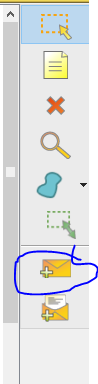
\includegraphics[width=\linewidth]{images/04.debugging-rete/06.png}
\end{center}

Finito il processo si potrà vedere visivamente il percorso del pacchetto, nel caso si voglia velocizzare il processo si può cliccare sul bottone Capture/Forward (o Fast Forward) presente sulla ,barra gialla in basso, il quale che velocizzerà il tutto.

Un' altra possibilità è quella che un dispositivo invii pacchetti a tutti, per farlo bisogna cliccare nell'altra icona della busta e cliccare sul dispositivo mittente, anche con questa soluzione bisognerà sistemare la event list e si potrà velocizzare il processo con il bottone Capture/Forward.

\begin{center}
    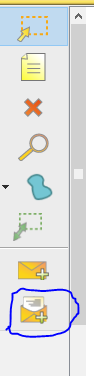
\includegraphics[width=\linewidth]{images/04.debugging-rete/07.png}
\end{center}

La seconda soluzione è consigliata all'inizio visto che è molto probabile che il software vi possa dare errore anche se nella rete non sono presenti errori, si consiglia di fare un paio di tentativi, all’inizio, con la seconda soluzione e poi potrete agire come meglio preferite.
